\chapter{Common blocks}
\label{chap:common}

%% Restart the numbering to make sure that this is definitely page #1!
\pagenumbering{arabic}

%% Quotes if we want to put them in 
\chapterquote{Laws were made to be broken.}%
{Christopher North, 1785--1854}%: Blackwood's Magazine May 1830

%% The defined macros should always be used
Once upon a time there was \chips which was very nice for \nova which like to use \unit{10}{\GeV} because
of \minos which was very naughty

%% Feynman diagrams
%% You have to use lualatex to get this working
\feynmandiagram [horizontal=a to b] {
i1 [particle=\(e^{-}\)] -- [fermion] a -- [fermion] i2 [particle=\(e^{+}\)],
a -- [photon, edge label=\(\gamma\), momentum'=\(k\)] b,
f1 [particle=\(\mu^{+}\)] -- [fermion] b -- [fermion] f2 [particle=\(\mu^{-}\)],
};

Symmetries, either intact or broken, have proved to be at the heart
of how matter interacts. The Standard Model of fundamental interactions
(SM) is composed of three independent continuous symmetry groups denoted
$\SUgroup{3} \times \SUgroup{2} \times \Ugroup{1}$, representing the
strong force, weak isospin and hypercharge
respectively~\cite{Phys.Rev.Lett.19.1264, Phys.Rev.D2.1285,hep-ph/0410370}.

\section{Neutral meson mixing}
\label{sec:neutralmixing}
We can go a long way with an effective Hamiltonian approach in
canonical single-particle quantum mechanics. To do this we construct
a wavefunction from a combination of a generic neutral meson state
$\ket{\Xzero}$ and its anti-state $\ket{\Xzerobar}$:

\begin{figure}
    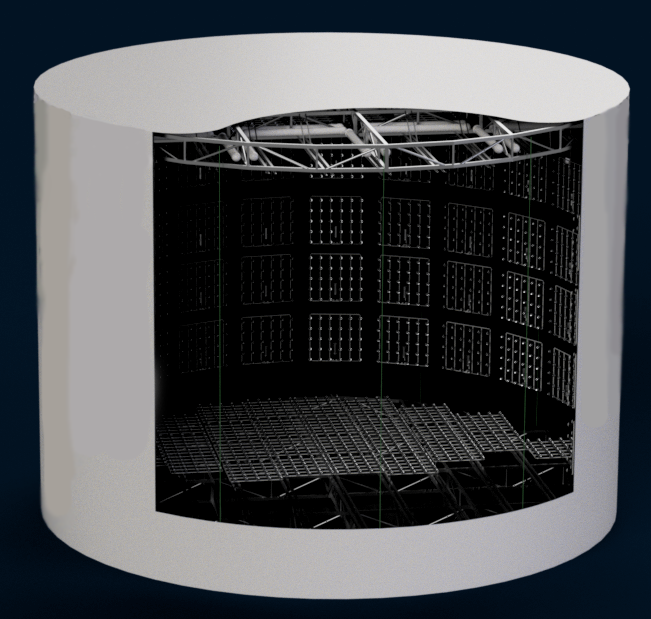
\includegraphics[width=\largefigwidth]{diagrams/chips_render_1}
    \caption[CKM Fitter constraints on \alphaCKM.]%
    {CKM Fitter constraints on \alphaCKM from combined \BToPiPi,
        \BToRhoPi and \BToRhoRho decay analyses.}
    \label{fig:chips_render_1}
\end{figure}

\begin{sidewaysfigure}
    \begin{center}
        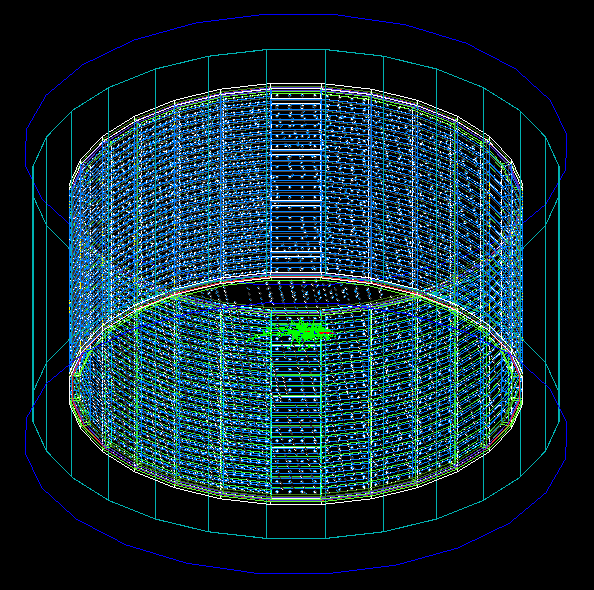
\includegraphics[width=0.8\textheight]{diagrams/chips_event}
        \caption[Cross-section view of \LHCb, cut in the non-bending $y$--$z$ plane]%
        {Cross-section view of \LHCb, cut in the non-bending $y$--$z$ plane.}
        \label{fig:chips_event}
    \end{center}
\end{sidewaysfigure}


Since both \bhadron{s} are preferentially produced in the same direction
and are forward-boosted along the beam-pipe, the detector is not required
to have full $4\pi$ solid-angle coverage. \LHCb takes advantage of this
by using a wedge-shaped single-arm detector with angular acceptance
\unit{10-300}{\mrad} in the horizontal (bending) plane~\cite{Amato:1998xt}.

\vspace{1cm}

\begin{center}
    {\hspace{1mm}\Large\vdots\hspace{1cm}}
\end{center}

\vspace{1cm}

The detector is illustrated in \FigureRef{fig:chips_render_1}, showing
the overall scale of the experiment.

%
\begin{equation}
    \ket{\psi(t)} = a(t)\ket{\Xzero} + b(t)\ket{\Xzerobar}
\end{equation}
%
which is governed by a time-dependent matrix differential equation,
%
\begin{equation}
    \I \pdByd{}{t} \colvector{a \\ b}
    =
    \underbrace{%
        \twomatrix{ M_{11}-\frac{\I}{2}\Gamma_{11}
            & M_{12}-\frac{\I}{2}\Gamma_{12} }
        { M_{12}^\ast-\frac{\I}{2}\Gamma_{12}^\ast
            & M_{22}-\frac{\I}{2}\Gamma_{22} }
    }_{\boldmatrix{H}}
    \colvector{a \\ b}
    .
\end{equation}

The single-sided detector design was chosen in preference to a two-armed
design since the detector dimensions are restricted by the layout of the
IP8 (ex-Delphi) cavern in which \LHCb is located. Using all the available
space for a single-arm spectrometer more than compensates in performance
for the \about{50\percent} drop in luminosity.

\section{The \Cerenkov mechanism}
A Huygens construction in terms of spherical shells of probability for photon
emission as the particle progresses along its track shows an effective
``shock-front'' of \Cerenkov emission. This corresponds to an emission cone of
opening angle \thetaCerenkov around the momentum vector for each point on the
track,
%
\begin{subequations}
    \label{eq:cosThetaCk}
    \begin{equation}
        \cos\,\thetaCerenkov  &= \frac{1}{n \beta} +
        \frac{\hbar k}{2p}%
        \parenths{ 1 - \frac{1}{n^2} } \\
        &\,\sim \frac{1}{n \beta}%
        \label{eq:cosThetaCkApprox}
    \end{equation}
\end{subequations}
%
where $\beta \equiv v/c$, the relativistic velocity fraction.

\section{Trigger system}
\label{sec:triggers}
An overview of the \LHCb trigger characteristics broken down by level
is shown in \Table~\ref{tab:TriggerDetails}.

\begin{table}[bp]
    \begin{tabular}{lllll}
                    & L0              & L1              & HLT             \\
        \midrule                                                          \\
        Input rate  & \unit{40}{\MHz} & \unit{1}{\MHz}  & \unit{40}{\kHz} \\
        Output rate & \unit{1}{\MHz}  & \unit{40}{\kHz} & \unit{2}{\kHz}  \\
        Location    & On detector     & Counting room   & Counting room   \\
    \end{tabular}
    \caption{Characteristics of the trigger levels and offline analysis.}
    \label{tab:TriggerDetails}
\end{table}

Here are some funky floats using ``continued captions'', i.e. for a semantically
collected group of float contents which are too numerous to fit into a single
float, such as the pretty circles in the following figure:

\newcommand{\circleimg}[1]{%
    \begin{tikzpicture}
        \draw[color=black,fill=#1,thick] (1,0) circle (1.5cm);
    \end{tikzpicture}%
}

\begin{figure}[hb]
    \subfloat[][Example 1a]{\label{fig:cc1a}\circleimg{red!80}}\quad
    \subfloat[][Example 1b]{\label{fig:cc1b}\circleimg{green!70!yellow}}\quad
    \subfloat[][Example 1c]{\label{fig:cc1c}\circleimg{blue!80}}\quad
    \subfloat[][Example 1d]{\label{fig:cc1d}\circleimg{orange!80!yellow}}
    \caption{Demonstration of \texttt{subfig} continued captions.}
    \label{fig:cc1}
\end{figure}

\begin{figure}[p]
    \ContinuedFloat
    \subfloat[][Example 1e]{\label{fig:cc1e}\circleimg{violet}}\quad
    \subfloat[][Example 1f]{\label{fig:cc1f}\circleimg{cyan}}\quad
    \subfloat[][Example 1g]{\label{fig:cc1g}\circleimg{magenta}}\quad
    \subfloat[][Example 1h]{\label{fig:cc1h}\circleimg{yellow}}
    \caption[]{Demonstration of \texttt{subfig} continued captions (continued).}
\end{figure}

\noindent
This mechanism means that the same float label is used for both pages of
floats. Note that we can refer to \FigureRef{fig:cc1} in general, or to
\FigureRef{fig:cc1g} on \PageRef{fig:cc1g} in particular!

\noindent
Just for the hell of it, let's also refer to \SectionRef{sec:neutralmixing}.

Here are some funky floats using ``continued captions'', i.e. for a semantically
collected group of float contents which are too numerous to fit into a single
float, such as the pretty circles in the following figure

\section{Convolutional Neural Networks}
\label{sec:cnn}

\section{CHIPS Events}
\label{sec:events}

\begin{figure}
    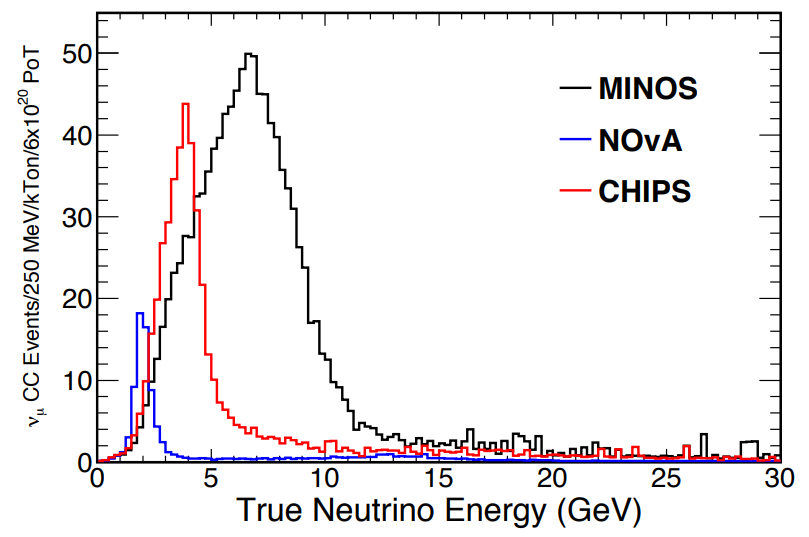
\includegraphics[width=\largefigwidth]{diagrams/numi_axis}
    \caption[CKM Fitter constraints on \alphaCKM.]%
    {CKM Fitter constraints on \alphaCKM from combined \BToPiPi,
        \BToRhoPi and \BToRhoRho decay analyses.}
    \label{fig:numi_axis}
\end{figure}

\begin{figure}
    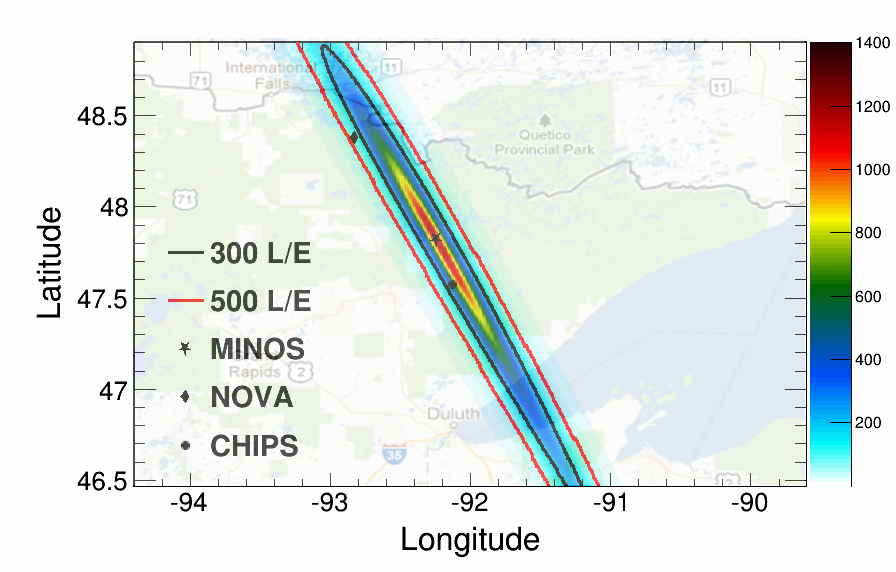
\includegraphics[width=\largefigwidth]{diagrams/numi_map}
    \caption[CKM Fitter constraints on \alphaCKM.]%
    {CKM Fitter constraints on \alphaCKM from combined \BToPiPi,
        \BToRhoPi and \BToRhoRho decay analyses.}
    \label{fig:numi_map}
\end{figure}

The expected beam flux at the CHIPS detector location is found from reweighting current

We can use current NuMI beam simulations

Current NuMI beam experiments


Once upon a time there was \chips which was very nice for \nova which like to use \unit{10}{\GeV}
